\documentclass[12pt]{article}

\usepackage[a4paper,margin=1in]{geometry}
\usepackage{graphicx}
\usepackage{amsmath}
\usepackage{booktabs}
\usepackage{listings}
\usepackage{xcolor}
\usepackage{hyperref}

\hypersetup{
    colorlinks=true,
    linkcolor=blue,
    urlcolor=blue
}

\lstset{
language=C,
basicstyle=\ttfamily\small,
keywordstyle=\color{blue},
commentstyle=\color{green!60!black},
stringstyle=\color{red},
numbers=left,
numberstyle=\tiny,
stepnumber=1,
numbersep=5pt,
frame=single,
breaklines=true,
showstringspaces=false
}

\begin{document}
\noindent
\begin{minipage}{0.6\textwidth}

\includegraphics[width=0.75\textwidth]{IIITB-COMET-Logo.png}
\end{minipage}
\begin{minipage}{0.38\textwidth}
\begin{center}
\textbf{DARSI VAMSI}
\newline
\textbf{COMET FWC 071}
\end{center}
\end{minipage}\\

\Large{\textbf{Implementation of Three LED Blinking using Direct GPIO Register Programming on the VAMAN ARM Development Board}}




\section{Objective}

The objective of this experiment is to understand the operation of General Purpose Input/Output (GPIO) registers by directly programming the GPIO peripheral of the VAMAN ARM Development Board. The experiment demonstrates sequential blinking of three LEDs using memory-mapped register access without relying on external hardware abstraction libraries.

\section{Hardware Requirements}

\begin{enumerate}
\item VAMAN ARM Development Board
\item USB Programming Cable
\item Ubuntu 24.04 LTS
\item Three On-board LEDs
\end{enumerate}

\section{Software Requirements}

\begin{enumerate}
\item GNU ARM Embedded GCC Compiler
\item Make Utility
\item Makefile
\item Text Editor (VS Code / Vim)
\item Terminal
\end{enumerate}

\section{Theory}

General Purpose Input Output (GPIO) is one of the most fundamental peripherals available in ARM-based microcontrollers. GPIO pins can be configured either as input pins for reading external signals or as output pins for driving external devices such as LEDs.

In this experiment, GPIO registers are accessed directly through memory-mapped addresses. The GPIO Direction Register configures the direction of each GPIO pin, while the GPIO Output Register controls the logic level present on the configured output pins.

The experiment avoids the use of any hardware abstraction library and directly manipulates the peripheral registers using pointers.

\section{GPIO Register Mapping}

\begin{table}[h]
\centering
\begin{tabular}{ccc}
\toprule
Register & Address Offset & Purpose\\
\midrule
GPIO\_DIR & 0x00 & Configure GPIO Direction\\
GPIO\_OUT & 0x04 & GPIO Output Register\\
\bottomrule
\end{tabular}
\caption{GPIO Register Description}
\end{table}

\section{LED Connections}

\begin{table}[h]
\centering
\begin{tabular}{cc}
\toprule
LED & GPIO Pin\\
\midrule
LED 1 & GPIO18\\
LED 2 & GPIO21\\
LED 3 & GPIO22\\
\bottomrule
\end{tabular}
\caption{GPIO Pins Used}
\end{table}

\section{Program Description}

The application begins by defining the base address of the GPIO peripheral and creating register definitions using volatile pointers.

Three GPIO pins (18, 21 and 22) are selected for controlling the LEDs.

Initially, the GPIO direction register is configured so that all three pins operate as output pins.

The program continuously performs the following operations:

\begin{enumerate}
\item Turn ON LED 1.
\item Wait using a software delay.
\item Turn OFF LED 1.
\item Turn ON LED 2.
\item Wait.
\item Turn OFF LED 2.
\item Turn ON LED 3.
\item Wait.
\item Turn OFF LED 3.
\item Repeat indefinitely.
\end{enumerate}

\section{Algorithm}

\begin{enumerate}
\item Define GPIO register addresses.
\item Configure GPIO18, GPIO21 and GPIO22 as output pins.
\item Enter an infinite loop.
\item Turn ON LED1.
\item Execute software delay.
\item Turn OFF LED1.
\item Turn ON LED2.
\item Execute software delay.
\item Turn OFF LED2.
\item Turn ON LED3.
\item Execute software delay.
\item Turn OFF LED3.
\item Repeat forever.
\end{enumerate}

\section{Source Code}



\section{Testing Procedure}

\begin{enumerate}
\item Compile the source code using the ARM GCC compiler.
\item Generate the executable binary.
\item Flash the binary into the VAMAN ARM Development Board.
\item Reset the development board.
\item Observe the three LEDs.
\item Verify that each LED glows one after another with a fixed delay.
\end{enumerate}

\section{Expected Output}

The LEDs blink in the following order:

\[
\boxed{\text{LED1} \rightarrow \text{LED2} \rightarrow \text{LED3} \rightarrow \text{Repeat}}
\]

Each LED remains ON for approximately the duration of the software delay before switching to the next LED.

\section{Observation}

\begin{itemize}
\item GPIO registers were successfully configured using direct memory-mapped register programming.
\item GPIO18, GPIO21 and GPIO22 functioned correctly as digital output pins.
\item Each LED blinked sequentially according to the program logic.
\item The software delay generated a visible blinking interval.
\item The experiment verified successful low-level GPIO programming on the VAMAN ARM Development Board.
\end{itemize}


\section{Advantages}

\begin{itemize}
\item Demonstrates low-level hardware programming.
\item Eliminates dependency on external libraries.
\item Provides better understanding of ARM peripheral registers.
\item Faster execution due to direct register access.
\item Useful for embedded systems and firmware development.
\end{itemize}


\section{Applications}

\begin{itemize}
\item Embedded System Development
\item Device Driver Development
\item GPIO Interface Testing
\item ARM Firmware Development
\item Hardware Validation
\item Industrial Automation
\end{itemize}


\section{Result}

The experiment was successfully implemented on the VAMAN ARM Development Board using direct GPIO register programming. The GPIO Direction Register and GPIO Output Register were configured correctly, allowing three LEDs connected to GPIO18, GPIO21 and GPIO22 to blink sequentially. The experiment verified the successful operation of memory-mapped GPIO control and demonstrated the fundamentals of low-level ARM embedded programming.\\
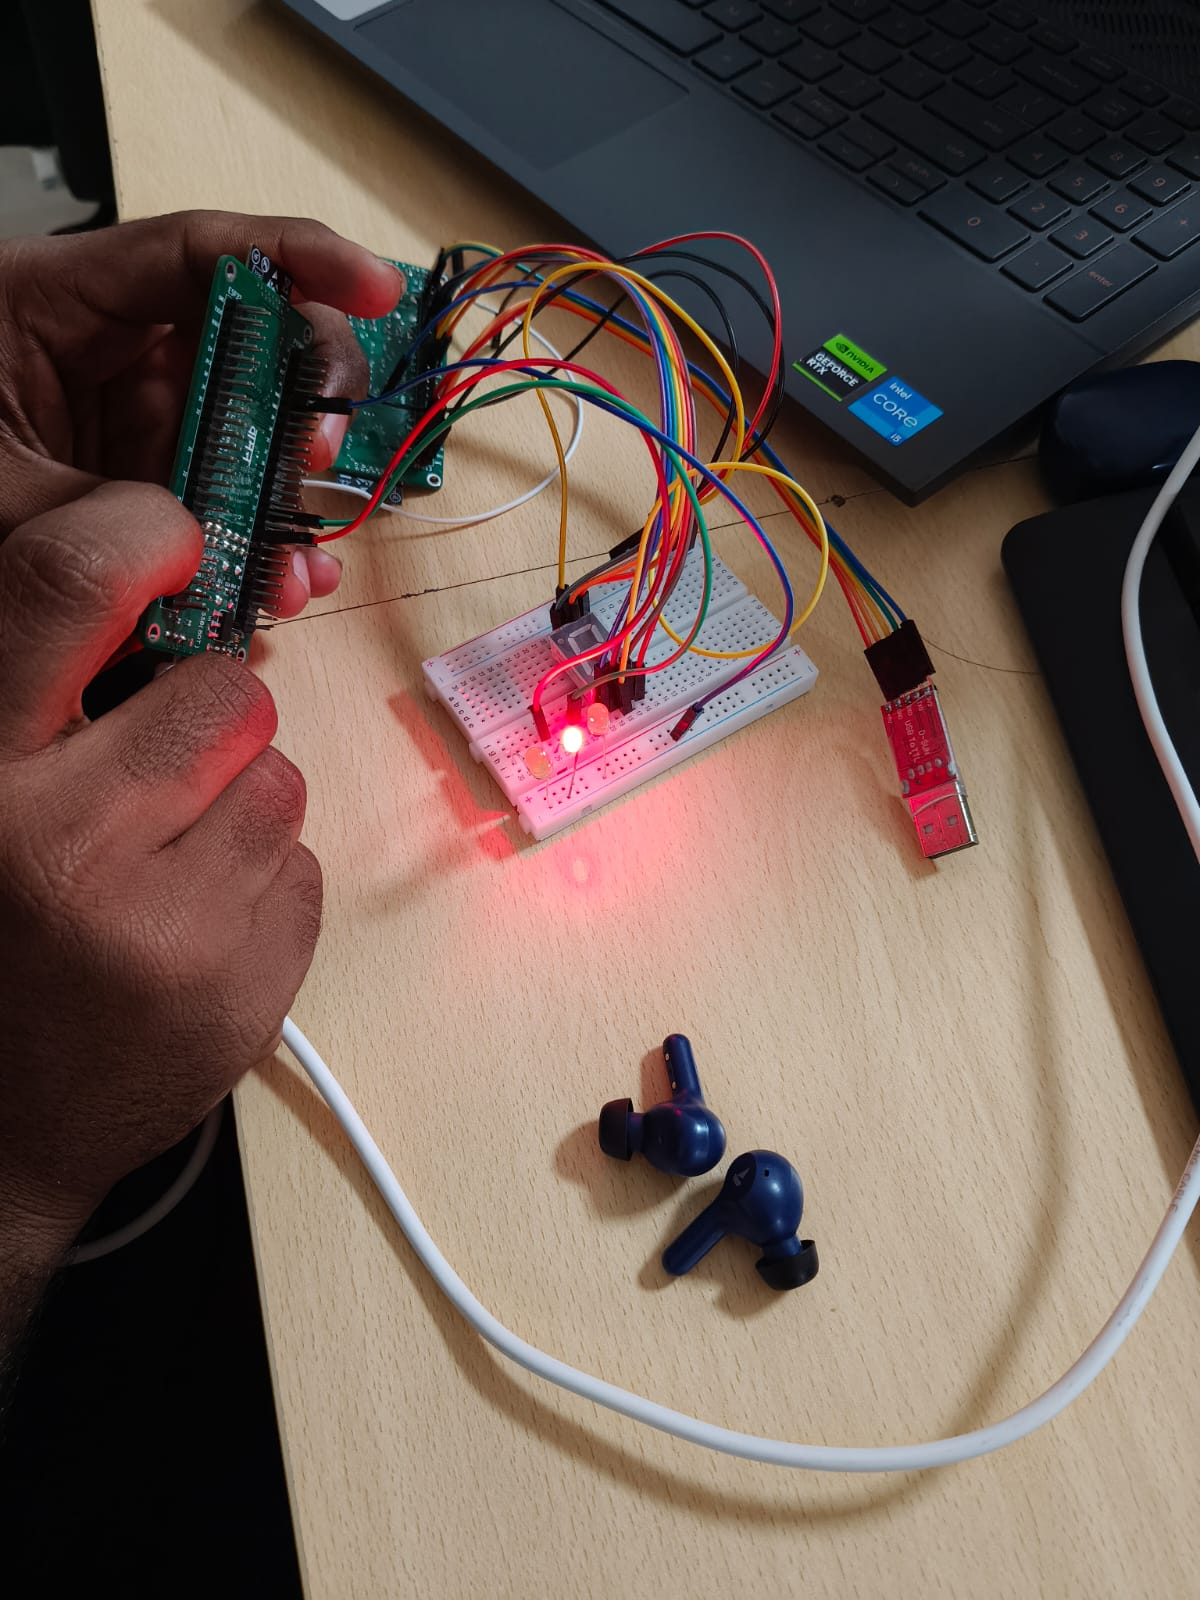
\includegraphics[width=0.75\textwidth]{Output_ledblink.png.jpeg}
\end{document}
